\section{Sub\-Bar\-Setting Class Reference}
\label{classSubBarSetting}\index{SubBarSetting@{SubBarSetting}}
{\tt \#include $<$subbarsetting.h$>$}

Inheritance diagram for Sub\-Bar\-Setting:\begin{figure}[H]
\begin{center}
\leavevmode
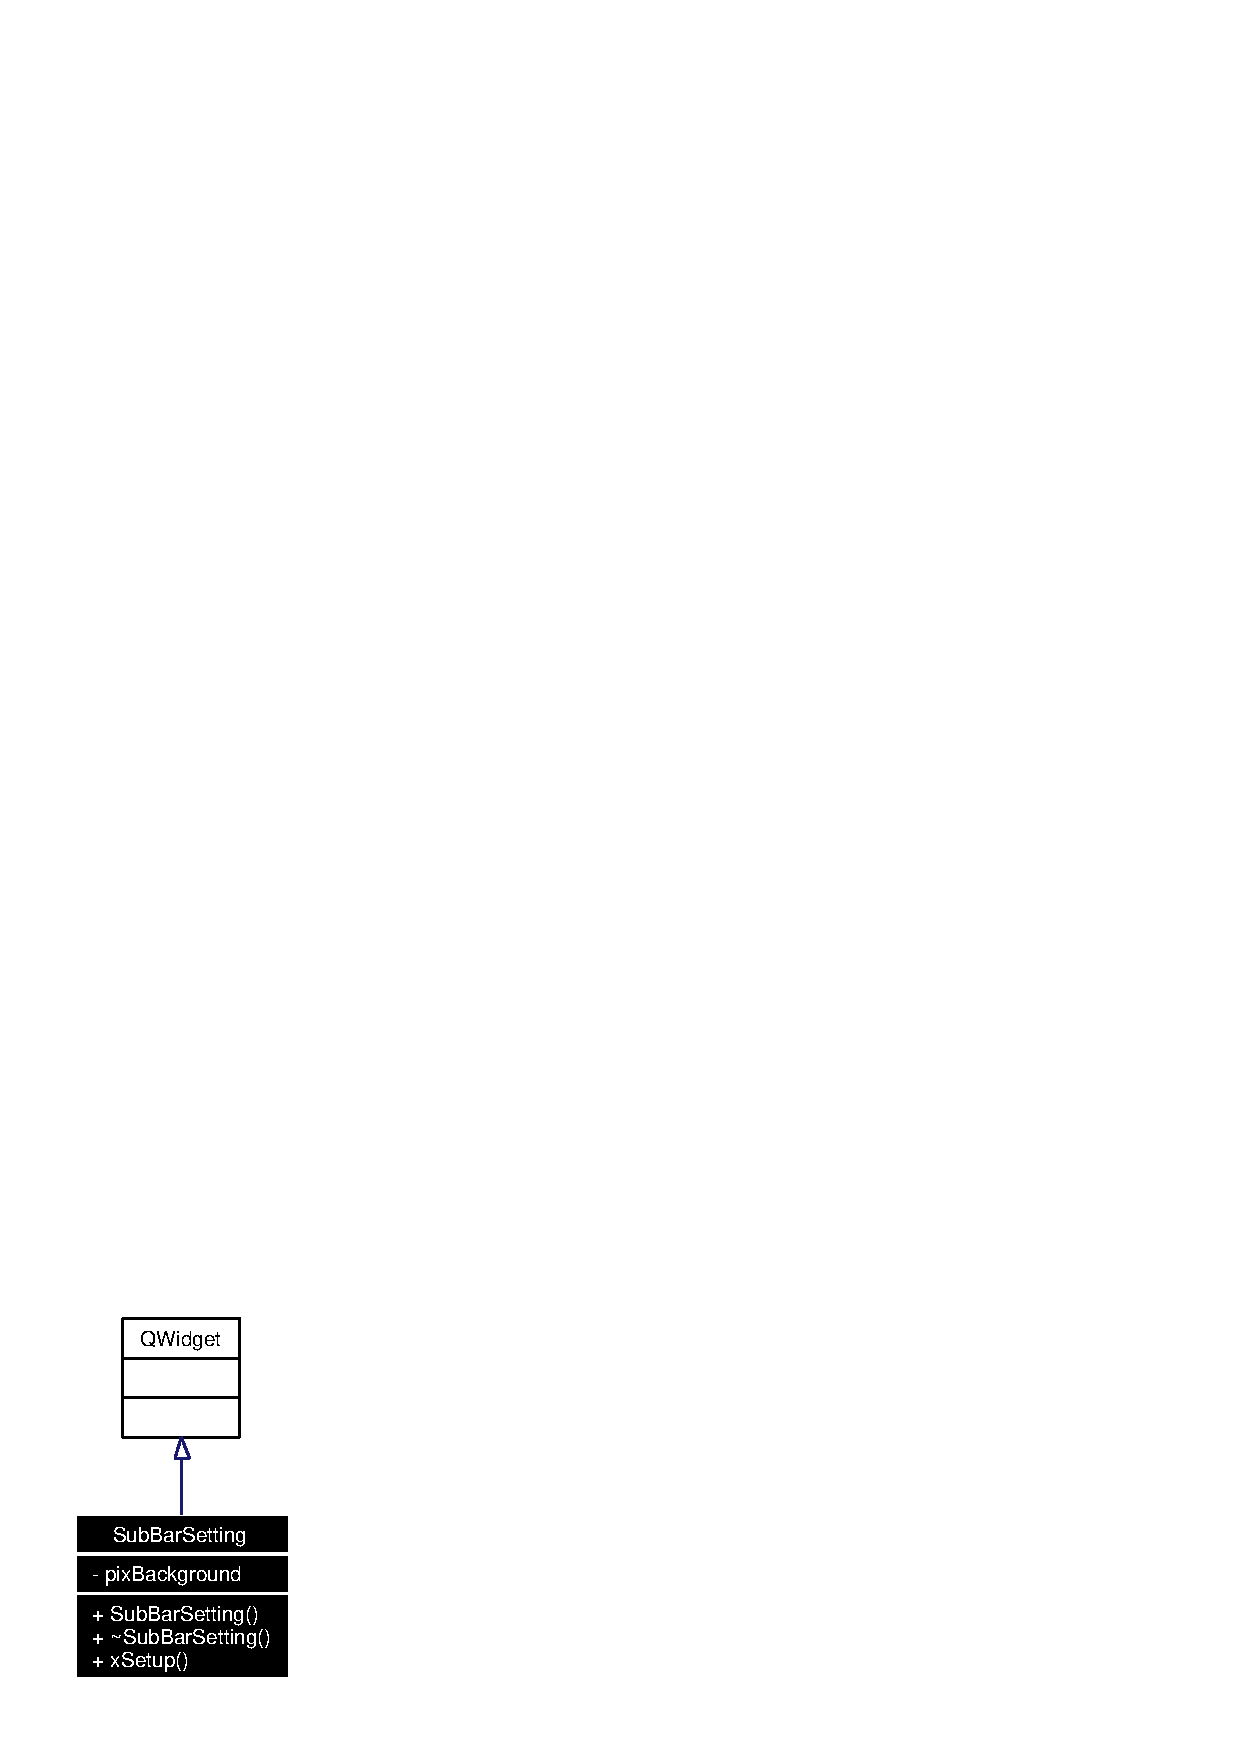
\includegraphics[width=69pt]{classSubBarSetting__inherit__graph}
\end{center}
\end{figure}
Collaboration diagram for Sub\-Bar\-Setting:\begin{figure}[H]
\begin{center}
\leavevmode
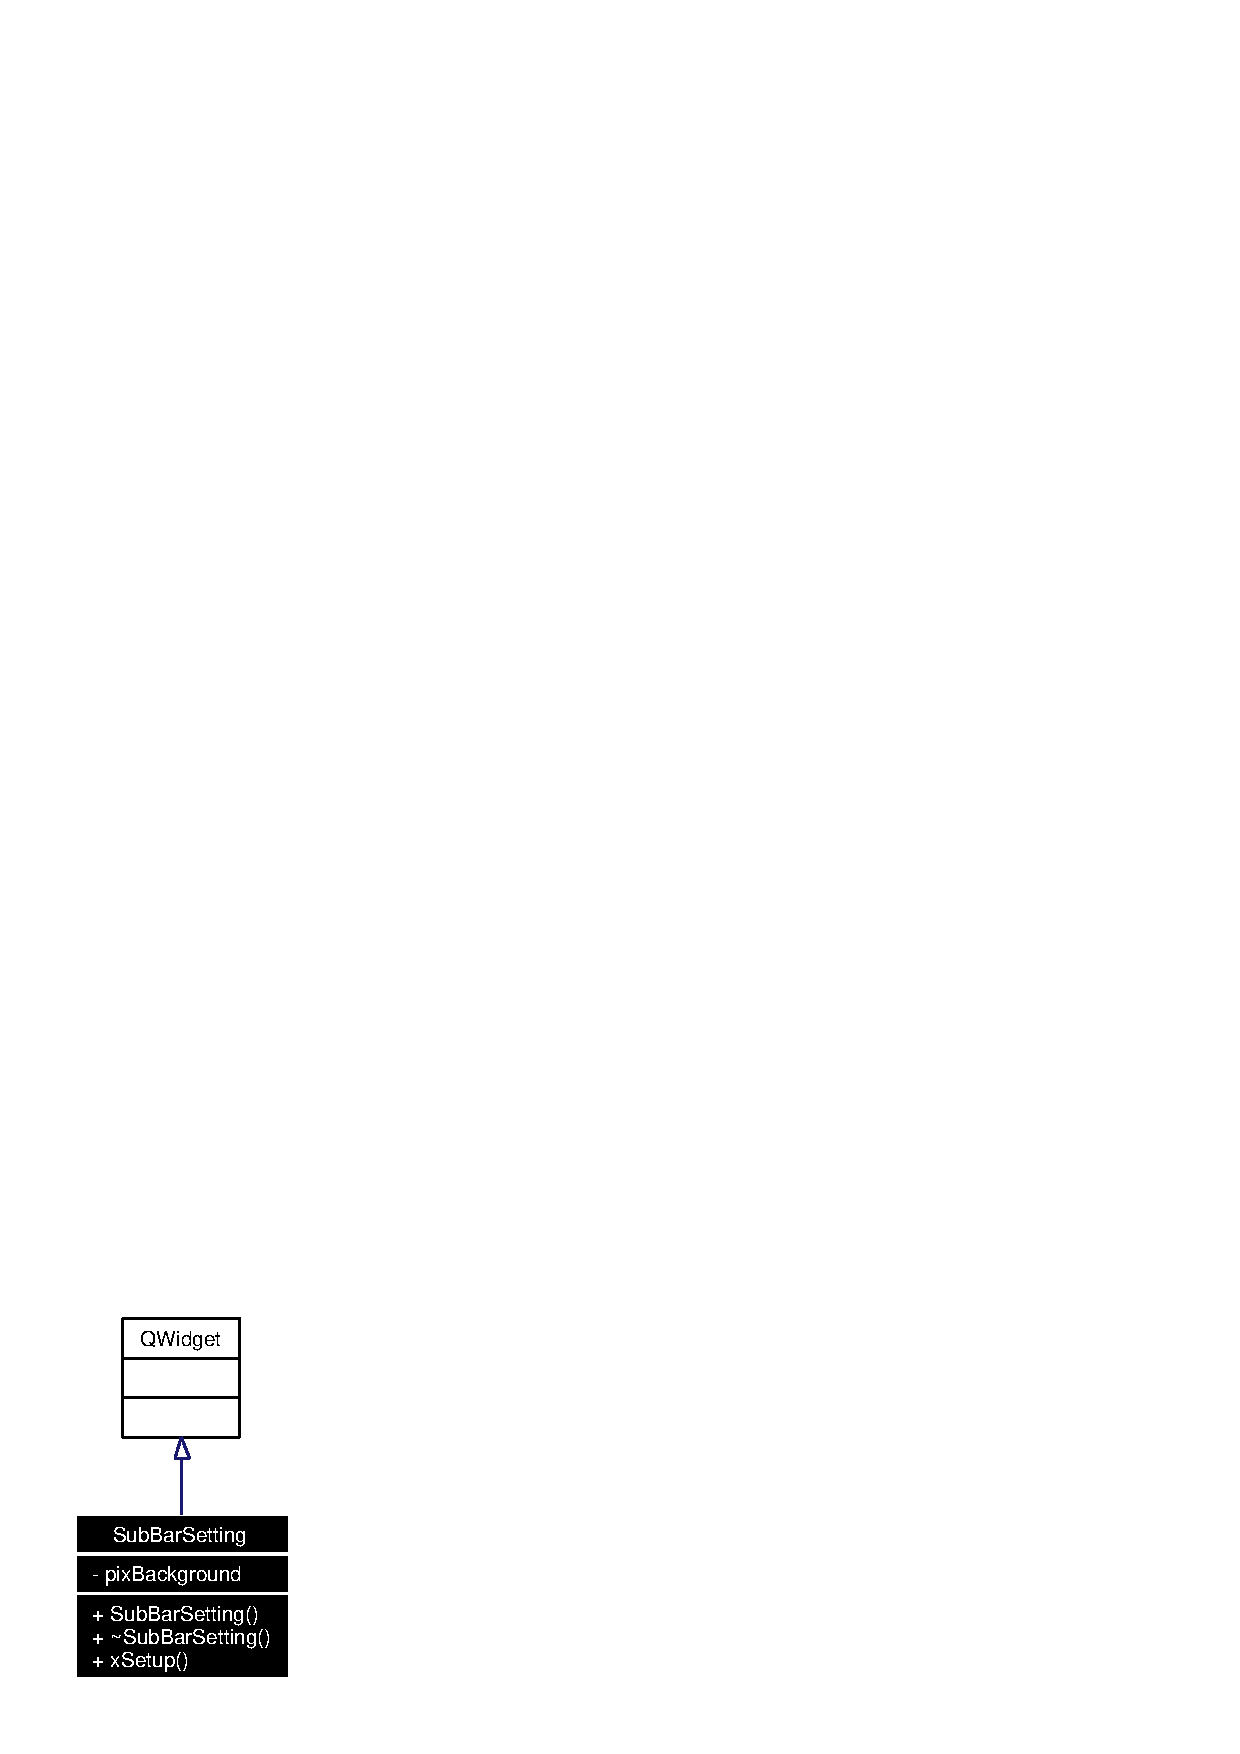
\includegraphics[width=69pt]{classSubBarSetting__coll__graph}
\end{center}
\end{figure}


\subsection{Detailed Description}
\begin{Desc}
\item[Author:]sonicat \end{Desc}




Definition at line 28 of file subbarsetting.h.\subsection*{Public Member Functions}
\begin{CompactItemize}
\item 
{\bf Sub\-Bar\-Setting} ({\bf QWidget} $\ast$parent=0, const char $\ast$name=0)
\item 
{\bf $\sim$Sub\-Bar\-Setting} ()
\item 
void {\bf x\-Setup} ()
\end{CompactItemize}
\subsection*{Private Attributes}
\begin{CompactItemize}
\item 
QPixmap {\bf pix\-Background}
\end{CompactItemize}


\subsection{Constructor \& Destructor Documentation}
\index{SubBarSetting@{Sub\-Bar\-Setting}!SubBarSetting@{SubBarSetting}}
\index{SubBarSetting@{SubBarSetting}!SubBarSetting@{Sub\-Bar\-Setting}}
\subsubsection{\setlength{\rightskip}{0pt plus 5cm}Sub\-Bar\-Setting::Sub\-Bar\-Setting ({\bf QWidget} $\ast$ {\em parent} = 0, const char $\ast$ {\em name} = 0)}\label{classSubBarSetting_SubBarSettinga0}




Definition at line 22 of file subbarsetting.cpp.

References x\-Setup().



\footnotesize\begin{verbatim}23  : QWidget(parent, name)
24 {
25   xSetup();
26 }
\end{verbatim}\normalsize 


Here is the call graph for this function:\begin{figure}[H]
\begin{center}
\leavevmode
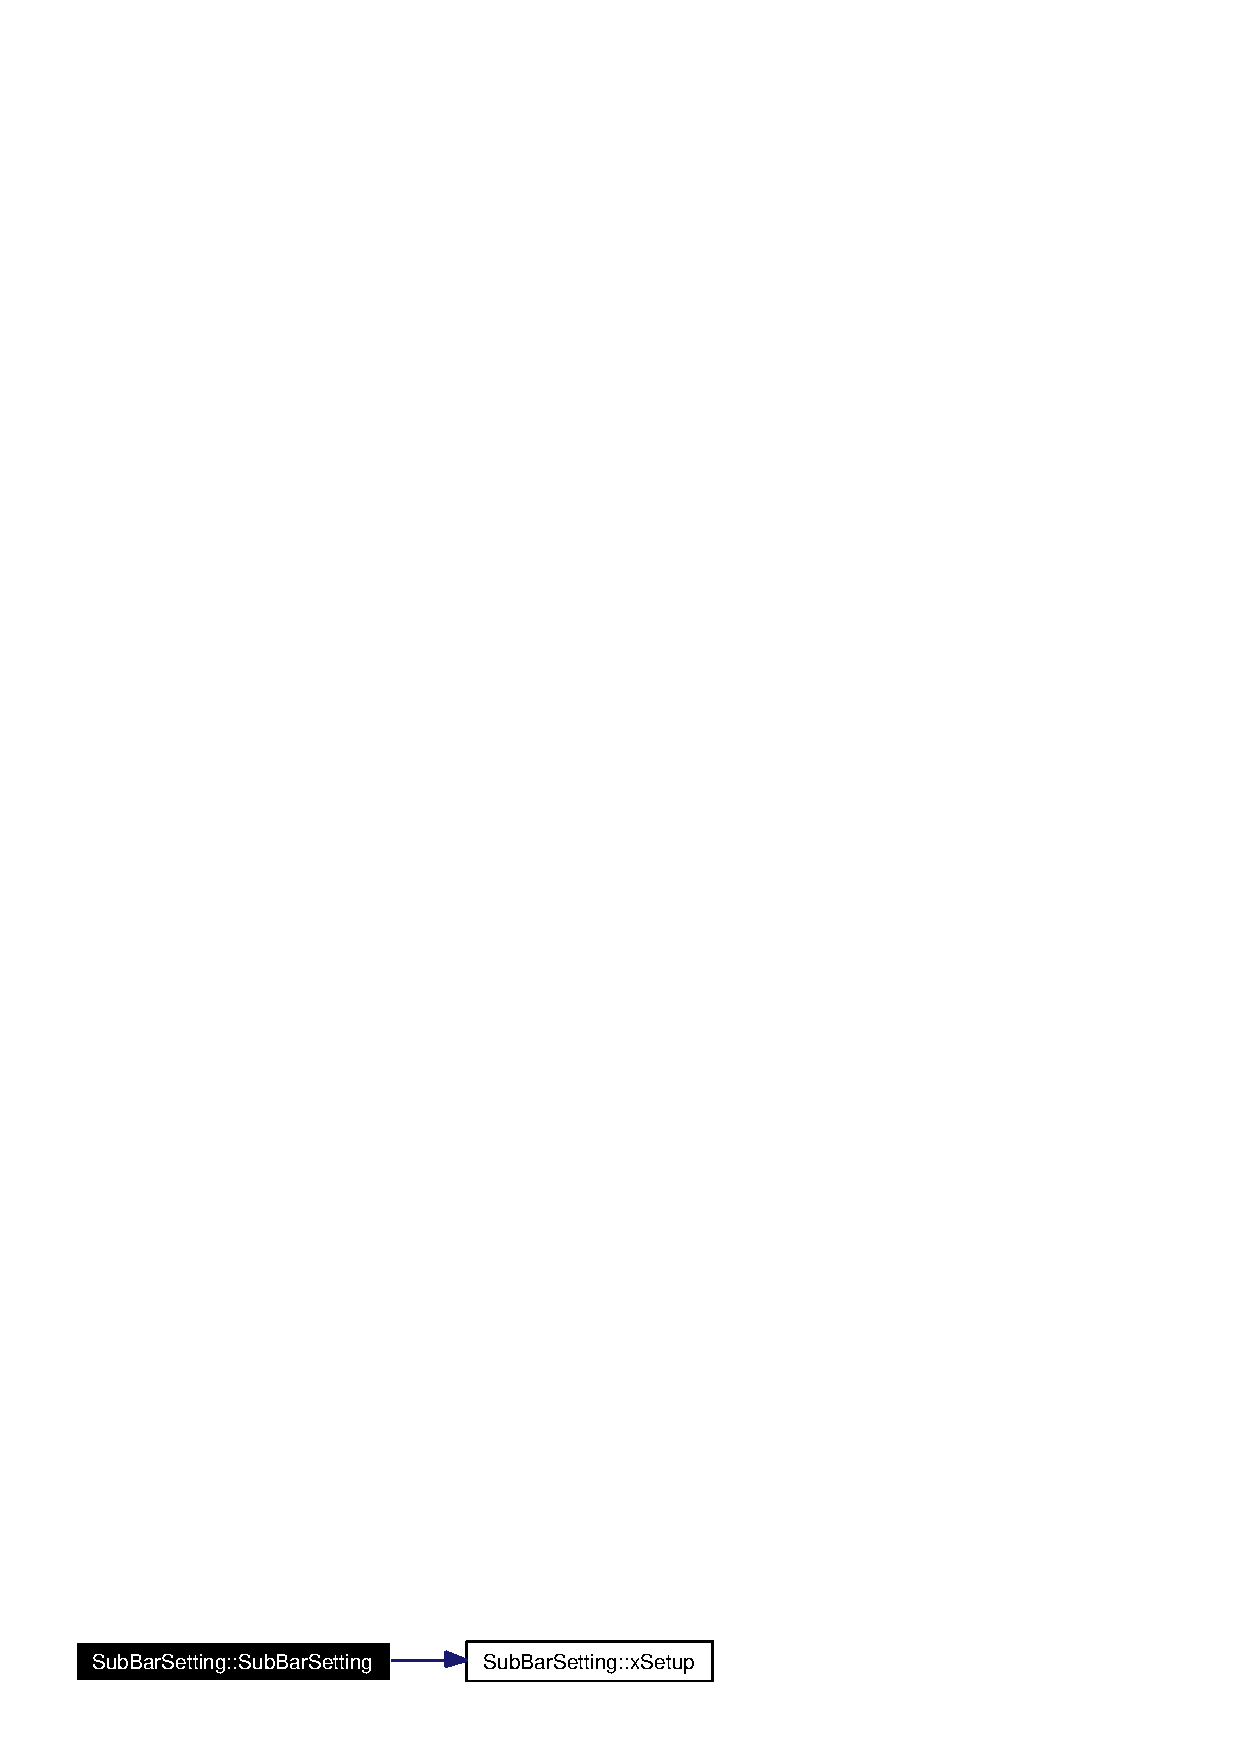
\includegraphics[width=171pt]{classSubBarSetting_SubBarSettinga0_cgraph}
\end{center}
\end{figure}
\index{SubBarSetting@{Sub\-Bar\-Setting}!~SubBarSetting@{$\sim$SubBarSetting}}
\index{~SubBarSetting@{$\sim$SubBarSetting}!SubBarSetting@{Sub\-Bar\-Setting}}
\subsubsection{\setlength{\rightskip}{0pt plus 5cm}Sub\-Bar\-Setting::$\sim${\bf Sub\-Bar\-Setting} ()}\label{classSubBarSetting_SubBarSettinga1}




Definition at line 29 of file subbarsetting.cpp.



\footnotesize\begin{verbatim}30 {
31 }
\end{verbatim}\normalsize 


\subsection{Member Function Documentation}
\index{SubBarSetting@{Sub\-Bar\-Setting}!xSetup@{xSetup}}
\index{xSetup@{xSetup}!SubBarSetting@{Sub\-Bar\-Setting}}
\subsubsection{\setlength{\rightskip}{0pt plus 5cm}void Sub\-Bar\-Setting::x\-Setup ()}\label{classSubBarSetting_SubBarSettinga2}




Definition at line 32 of file subbarsetting.cpp.

Referenced by Sub\-Bar\-Setting().



\footnotesize\begin{verbatim}33 {
34    //DAVID Setup Background;
35    pixBackground.load("/root/kde_application/hdass08/skin/SubBarBackground.png");
36    setBackgroundPixmap(pixBackground);
37 }
\end{verbatim}\normalsize 


\subsection{Member Data Documentation}
\index{SubBarSetting@{Sub\-Bar\-Setting}!pixBackground@{pixBackground}}
\index{pixBackground@{pixBackground}!SubBarSetting@{Sub\-Bar\-Setting}}
\subsubsection{\setlength{\rightskip}{0pt plus 5cm}QPixmap {\bf Sub\-Bar\-Setting::pix\-Background}\hspace{0.3cm}{\tt  [private]}}\label{classSubBarSetting_SubBarSettingr0}




Definition at line 37 of file subbarsetting.h.

The documentation for this class was generated from the following files:\begin{CompactItemize}
\item 
{\bf subbarsetting.h}\item 
{\bf subbarsetting.cpp}\end{CompactItemize}
